%==============================================================================
% Appendix B: Full response inventories
%==============================================================================
\section{Full Response Inventories}
\label{app:B}

This appendix collects the full response inventories that appear in
summary form in the body.  Where the body compresses the tables for
readability, here the tables are gathered together for ease of comparison.

\subsection{Bulk Inventory}
\label{app:B:bulk}

\begin{table}[H]
\centering
\resizebox{\linewidth}{!}{%
\begin{tabular}{lcccc}
\toprule
Entry & $\Tthree$ & $\Nilthree$ & $\Sthree$ & $\Solthree$ \\
\midrule
Maxwell coefficient & $-L^2/(2 r_0^4)$ & $-L^2/(2 r_0^4)$ & $-L^2/(2 r_0^4)$ & $-L^2/(2 r_0^4)$ \\
CS direction count & 0 & 1 & 3 & 0 \\
KK Higgsing & none & uniaxial & triaxial & biaxial \\
EC slice minimum & absent & present & absent & present \\
spin-2 rigidity & non-rigid & non-rigid & non-rigid & rigid \\
$P$-linear transport & protected & activated & activated & protected \\
nonlinear opening & absent & absent & activated & absent \\
defect-localisation response ($\eta$ benchmark) & trivial & activated & activated & EC-supported / CS-inert \\
inhomogeneous bulk response & trivial & activated & activated & CS-inert / EC-active \\
\bottomrule
\end{tabular}%
}
\caption{Full bulk inventory.}
\label{tab:appB_bulk}
\end{table}

\begin{figure}[H]
\centering
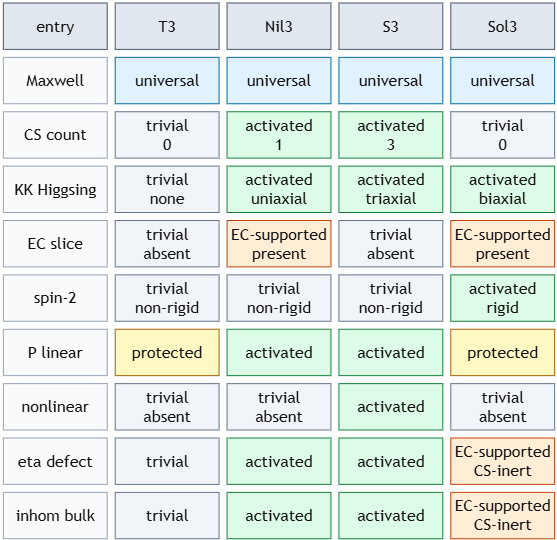
\includegraphics[width=0.95\linewidth]{figures/fig08_bulk_inventory_block.png}
\caption{36-entry bulk inventory block diagram.  The 9 entries $\times$ 4
geometries of \S\ref{app:B:bulk} are colour-coded as
\texttt{universal / activated / protected / trivial / EC-supported}.  In
particular, $\Solthree$ shares CS count $0$ with $\Tthree$, but in the EC
slice and inhomogeneous response rows it branches to the EC-supported side.}
\label{fig:bulk_block}
\end{figure}

The bulk inventory takes the form ``universal baseline + geometry-dependent
activation''.  $\Nilthree$ and $\Sthree$ progress as far as a local
parity-odd response on the activated side; $\Tthree$ is the minimal / inert
benchmark.  $\Solthree$ is CS-inert in the direction count but carries an EC
slice minimum and a rigid scaffold, so it is not placed in the same minimal
class as $\Tthree$.  The row ``defect-localisation response ($\eta$
benchmark)'' records not the existence of a bound state in the common
reduced 1D $\eta$-benchmark but how the localisation links to the additional
structure.

\subsection{Boundary Inventory}
\label{app:B:boundary}

\begin{table}[H]
\centering\small
\begingroup
\renewcommand{\arraystretch}{2.0}
\begin{tabularx}{\linewidth}{YXXXX}
\toprule
Entry & $\Tthree$ & $\Nilthree$ & $\Sthree$ & $\Solthree$ \\
\midrule
CS interface jump & absent & present & present & absent \\
APS spectral entry & $0$ & strict $+1/2$\newline (local) & $0$ & $0/1$\newline (Sol-A / Sol-P) \\
frame-bundle-norm. torsional charge $\Ntop$ & 0 & 0 & $6 r_0^2$ & 0 \\
CZ inflow & absent & activated & activated & absent \\
edge / interface response & minimal & activated & activated & spin-sensitive \\
boundary tag & trivial\newline benchmark & APS local\newline core & torsional-\newline charge active & global spectral\newline branch \\
\bottomrule
\end{tabularx}
\endgroup
\caption{Full boundary inventory.}
\label{tab:appB_boundary}
\end{table}

The strict observable of $\Nilthree$ belongs to the local spectral family,
that of $\Sthree$ to the torsional-charge family.  Furthermore, on the
compact mapping-torus benchmark, $\Solthree$ may carry a global spectral
branch.  This distinction is the key to understanding the mixed pairs and
source differences in the pairwise dictionary.

\subsection{Pairwise Cobordism Dictionary}
\label{app:B:pairwise}

\begin{table}[H]
\centering\small
\begingroup
\renewcommand{\arraystretch}{1.5}
\begin{tabularx}{\linewidth}{lXXX}
\toprule
Pair & Class & Dominant observable & Not-comparable note \\
\midrule
$\Sthree \leftrightarrow \Tthree$ & torsional / trivial & frame-bundle-norm.\ torsional charge & none \\
$\Sthree \leftrightarrow \Nilthree$ & torsional / local spectral & mixed & torsional-charge and local spectral are not the same quantity \\
$\Sthree \leftrightarrow \Solthree$ & torsional / global spectral & spin-sensitive & torsional-led for Sol-A; mixed for Sol-P \\
$\Tthree \leftrightarrow \Nilthree$ & trivial / local spectral & spectral & none \\
$\Tthree \leftrightarrow \Solthree$ & trivial / global spectral & spin-sensitive & Sol-A: trivial;\newline Sol-P: global spectral \\
$\Nilthree \leftrightarrow \Solthree$ & local / global spectral & spectral & source distinction within the spectral family \\
\bottomrule
\end{tabularx}
\endgroup
\caption{Full pairwise cobordism dictionary.}
\label{tab:appB_pairwise}
\end{table}

In the pairwise table the dominant observable supplies the subject of
comparison, and the ``not-comparable note'' makes explicit either that
direct subtraction is meaningless because the observable families differ,
or that the source differs even within the same spectral family.

\subsection{Strict Normalisation Cores}
\label{app:B:cores}

Together with the boundary observable families, the principal results of
this paper are supported by three strict normalisation cores.  These appear
in the reduced-side consistency statements of \S\ref{sec:circle:kk} but do
not define new second-layer observable families; they are native
quantities that guarantee the internal consistency of the Euclidean
response dictionary.

\begin{table}[H]
\centering\small
\begingroup
\renewcommand{\arraystretch}{1.5}
\begin{tabularx}{\linewidth}{clXYp{3.5cm}}
\toprule
\# & Core statement & Descriptor & Status & Verification \\
\midrule
C-1 & $k_{3D}^{\mathrm{tor\text{-}CS}} = \tfrac{1}{2}\,k_{4D}^{\NY}$ & $\Ctor$ inflow normalisation & strict (CZ + Stokes) & \S\ref{app:E:E11} \\
C-2 & $Q_{\mathrm{best}} = 1$ & doubly normalisation-free quotient & strict (matter assumption minimal) & \S\ref{app:E:E12} \\
C-3 & $k_q\in\mathbb{Z}$ & reduced CS level integrality & formal (single-valuedness) & \S\ref{app:E:E13} \\
\bottomrule
\end{tabularx}
\endgroup
\caption{Three strict normalisation cores.}
\label{tab:appB_cores}
\end{table}

\subsubsection{KK Reduction Normalisation Identity (C-1)}
\label{app:B:C1}

For the 4D Nieh--Yan action
$S_\NY^{(4D)} = (k_{4D}^{\NY}/8\pi^2)\int_{X^4}\mathrm{NY}$, applying the CZ
identity $\mathrm{NY} = \dd\Ctor$ together with Stokes' theorem on
$X^4 = M^3\times[0,\beta]$ gives, on the 3D boundary,
\begin{equation}
  S_{\mathrm{eff}}^{(3D)} \supset \frac{k_{4D}^{\NY}}{2}\cdot \Ntop.
\end{equation}
Hence the coefficient on the normalised basis
\begin{equation}
  \Ntop := \frac{1}{4\pi^2}\int_{M_3}\Ctor
\end{equation}
is fixed as the 3D torsion-CS coefficient,
\begin{equation}
  k_{3D}^{\mathrm{tor\text{-}CS}} = \frac{1}{2}\,k_{4D}^{\NY}.
\end{equation}
Here $\Ntop$ stands for the basis of the frame-bundle-normalised torsional
charge; since this paper imposes no extra quantisation condition on $r_0$,
no general integrality is claimed.  The factor $1/2$ originates from
$4\pi^2/8\pi^2$ and is independent of $r_0$.  Furthermore, on the untwisted
product circle the parity-odd residue from a real bosonic KK decomposition
takes the form $n\,w(n^2)$, so the contribution of the KK tower
($n\neq 0$) cancels strictly in pairs.  Detailed derivation and SymPy
verification are in Appendix~\ref{app:E:E11} and
\texttt{proofs/kk\_normalization.py}.

\subsubsection{Matter-Minimal Inflow Audit (C-2)}
\label{app:B:C2}

The quotient $Q_{\mathrm{best}} = \eta(0)/\Delta k_{\mathrm{matter}}$ is
formed from the numerator $\eta(0)^{(3D)} = 1$ (\S\ref{app:E:E10}) and the
denominator $\Delta k_{\mathrm{matter}} = h_{\mathrm{rep}}/2 = 1$
(Redlich parity shift \cite{Redlich1984}, $h_{\mathrm{rep}} = 2$).  Both are
\emph{doubly normalisation-free}:

\begin{itemize}
  \item the numerator is a spectral invariant that does not pass through
        the 4D APS bridge;
  \item the denominator depends only on $h_{\mathrm{rep}}$ and does not pass
        through the KK normalisation.
\end{itemize}

Hence $Q_{\mathrm{best}} = 1$ is a strict invariant independent of
normalisation conventions.  Details are in Appendix~\ref{app:E:E12}.

\begin{remark}
The Redlich parity shift is used here only as the standard
three-dimensional normalisation unit for the parity-odd level shift.
No dynamical fermion field is introduced in the geometric sector,
and the comparison is kept at the level of a translation-layer
normalisation audit.
\end{remark}

\subsubsection{Formal Quantisation on the Frame Bundle (C-3)}
\label{app:B:C3}

For the parity-odd effective action
$S_{\mathrm{odd}}^{(3D)} = k_q\cdot W[A/\omega]$ on the 3D boundary, the
single-valuedness $e^{i\Delta S_{\mathrm{odd}}} = 1$ requires, for the unit
winding shift under a large rotation on the frame bundle
($\pi_3(SO(3)) = \mathbb{Z}$),
\begin{equation}
  e^{2\pi i k_q} = 1 \iff k_q \in \mathbb{Z}.
\end{equation}
This gives a formal quantisation condition for the boundary Chern--Simons
level associated with the frame-bundle response. In the present work, this
condition is used as a boundary-level consistency criterion. Its complete
identification with the four-dimensional Nieh--Yan coupling
$\theta_{\rm NY}$ requires an additional normalization bridge between the
four-dimensional Nieh--Yan transgression and the three-dimensional
frame-bundle Chern--Simons functional. That bridge is not fixed here.
Accordingly, the statement $k_q\in\mathbb{Z}$ should be read as a formal
boundary quantisation condition, rather than as a first-principles derivation
of the $\theta_{\rm NY}$ normalization. Details are in Appendix~\ref{app:E:E13}.

\subsubsection{Cross-Audit Summary}
\label{app:B:cross}

C-1, C-2, and C-3 are cross-audited along three independent routes.  Here
``independent'' is restricted to the meaning ``no core uses the value of
another as input''.  Normalisation conventions such as $1/(4\pi^2)$,
$1/(8\pi^2)$, and $T_R = 1$ may be shared across cores, but this is a
common convention layer rather than circulation.  The inputs to each core
are listed below.

\begin{table}[H]
\centering\small
\begingroup
\renewcommand{\arraystretch}{1.5}
\begin{tabularx}{\linewidth}{@{}lY@{\hspace{1.2em}}Yc@{}}
\toprule
Core & Input from & \shortstack{Physical\\quantities} & \shortstack{Depends on\\other core?} \\
\midrule
C-1: $k_{3D}^{\mathrm{tor\text{-}CS}} = k_{4D}^{\NY}/2$ & 4D NY action + CZ + Stokes & $\Ctor$, $\Ntop$ basis & NO \\
C-2: $Q_{\mathrm{best}} = 1$ & spinor APS ($\eta(0) = 1$) + Redlich shift ($h_{\mathrm{rep}} = 2$) & $\Csig$ & NO \\
C-3: $k_q\in\mathbb{Z}$ & path-integral single-valuedness + $\pi_3(SO(3))$ & frame-bundle data & NO \\
\bottomrule
\end{tabularx}
\endgroup
\caption{No-circulation cross-audit summary.}
\label{tab:appB_cross}
\end{table}

C-1 belongs to the torsional sector ($\Ctor$), C-2 to the spectral sector
($\Csig$), and C-3 to formal frame-bundle quantisation; none uses another's
value as input.  This is the meaning of ``no circulation''.  The minimality
of the matter assumption appears only in $h_{\mathrm{rep}} = 2$ of C-2, and
the complete identification between the native and translation-layer
quantities is left outside the scope of this paper.

\subsection{Selection-Rule Catalogue}
\label{app:B:rules}

Although the body presents a compact summary, the rule catalogue can be
read in the following four clusters.  Here R1--R5 are the bulk-rule labels
introduced in \S\ref{sec:rules:bulk}, and B1--B4 are the boundary-rule
labels of \S\ref{sec:rules:boundary}.

\begin{table}[H]
\centering
\begingroup
\renewcommand{\arraystretch}{1.5}
\begin{tabularx}{\linewidth}{YlY}
\toprule
Cluster & \shortstack{Representative\\rules} & Content \\
\midrule
bulk universality\newline cluster & R1 &
  geometry-independence of the Maxwell baseline \\
bulk activation\newline cluster & R2--R5 &
  branching of CS, Higgsing, EC slice minimum, reduced $\eta$-benchmark response \\
boundary family\newline cluster & B1--B4 &
  inflow / local spectral core / torsional-charge / spectral-source distinction \\
pairwise comparison\newline cluster & \S\ref{sec:rules:pairwise} &
  pairwise dominant observable and mixed pairs \\
\bottomrule
\end{tabularx}
\endgroup
\caption{Four clusters of selection rules.}
\label{tab:appB_clusters}
\end{table}

This catalogue allows the rule set in the body to be re-read from the
viewpoint of ``what is universal and what is geometry-dependent''.
